\chapter{Spectroscopy \& Fluorescence in Chlorophyll}
\thispagestyle{fancy}
\fancyhead[RE,LO]{Experiment \thechapter}
Fluorescence is one of the possible mechanisms for emission of light by a substance that has absorbed light. 
It sounds simple. 
Light goes in, light comes out. 
So how is fluorescence different from other types of emission? 
The important thing to remember about fluorescence is that the emitted photon of light will be lower energy (will have a longer wavelength) than the photon of light that was initially absorbed. 
You are probably familiar with some objects that display fluorescence, such as glow-in-the-dark T-shirts that glow under ultraviolet (UV) light sources. 
The reason that these materials appear to “glow” is that they are able to absorb UV light (which the human eye cannot see) and re-emit it as light of a longer wavelength in the visible spectrum (which we can see!). 
Fluorescent materials give our eyes access to light that would normally be invisible to us by direct absorption-emission processes. 
But not all fluorescent processes or materials require UV light. 
Some, like chlorophyll, can absorb light in the violet/blue region and emit light in the red region. 
%
\begin{wrapfigure}{r}{0.44\textwidth}
  \vspace{-15pt}  
  \begin{center}
    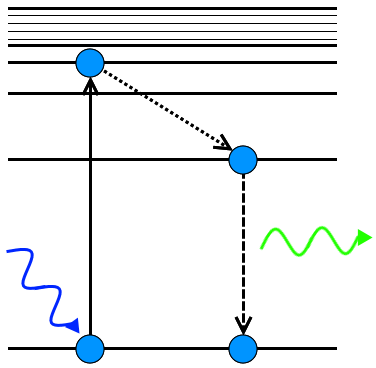
\includegraphics[width=0.42\textwidth]{fluorescence}
  \end{center}
  \vspace{-20pt}
  \caption{Simple model of fluorescence.}
  \label{fig:fluorescence}
  \vspace{-5pt}
\end{wrapfigure}
%
As you may have seen before in a biology course, if a violet or blue light is shone through a sample of spinach extract, the solution turns red in color.
\par 
You, the astute student, might ask, “Well, if the emitted photon is lower in energy than the absorbed photon, what happened to the rest of the energy?” 
Excellent question. 
The answer lies in the combination of two different types of energy levels for molecules: electronic states and vibrational states. 
Electronic states deal with the energy levels of electrons, which are excited by photon absorption and relaxed by photon emission. 
Vibrational states deal with the periodic motion of the atoms of the molecule, just like the mass-spring model that you have already studied for HCl molecules. 
For each electronic state there are multiple vibrational states that a molecule can assume. 
So each electronic energy level gets split into many nearby levels. 
Transitions between these nearby vibrational energy levels tend to involve interactions with other molecules or atoms, whereas electronic transitions between groups of levels tend to involve photons. 
This is modeled in the figure~\ref{fig:fluorescence}, where an incoming blue photon is absorbed, causing a transition from ground state into the highest vibrational level of the 1st excited state. 
The molecule then undergoes several transitions between vibrational levels, essentially sharing the vibrational energy with neighboring atoms or molecules, a process which takes a few picoseconds, comparable to the typical time for vibrations between atoms.
The molecule remains at this equilibrium vibration level for a ``long'' time — plenty of time to reach true equilibrium in its vibrations but short compared to our everyday experience (typically several nanoseconds) — before returning back to the ground level, emitting a green photon.
\par 
In this one-week lab, you will be working with chlorophyll to explore fluorescence. 
Chlorophyll is a fluorescent substance. 
Chlorophyll absorbs light in the UV, violet, and blue regions of the EM spectrum and fluoresces in the red region. 
The intensity of the red color is a function both of how much chlorophyll is in the sample and of what light source is used to excite the chlorophyll. 
Chemical compounds that exhibit fluorescence are commonly called fluorophores (or fluorochromes).
\par 
Your lab will consist of two parts: I) examining the fluorescence of chlorophyll, and II) considering physical implications of the ways in which fluorescence is presented in other science venues. 
The lab report you turn in at the end of today's lab should discuss answers to questions posed in the sections below as well as any insights you gain from your explorations and investigations, along with the data supporting those insights.

\section*{Equipment:}
Each group has access to:
\begin{itemize}
\itemsep-0.3em
\item a spectrometer and fiber optic cable (BE GENTLE WITH THE CABLE—no bending, no crushing) that can interface with the computer via a USB port,
\item Logger Pro software for the computer,
\item a small stand with multiple 90-clamps,
\item a UV light source,
\item small LED light boxes emitting different colors of light (Red, Green, and Blue), and
\item a light ray box (with an incandescent bulb that acts as a white light source).
\end{itemize}

\section*{Part I: Examining the Fluorescence of Chlorophyll}
To collect the fluorescence produced when chlorophyll is illuminated by UV/violet/blue
light, you will want to consider how to set up the system of light source, chlorophyll sample, and
fiber optic cable (detector). Here are some questions you might need to consider in order to collect
this data:
\begin{itemize}
\itemsep-0.3em
\item What type of light source should you use?
\item Do you want to see if more than one source can cause fluorescence for the chlorophyll?
\item Do you want the fiber optic cable (detector) to point through the chlorophyll sample at the light source (all in a line), or would it be better to have the detector directed perpendicular to the light source? Or is there some other set up that is better? What are the advantages and disadvantages of these methods?
\item Do you expect the intensity (brightness) of the fluorescent light to be high or low? Do you think the overhead (classroom) lights will interfere? What about the ambient light from the classroom window?
\end{itemize}
Once you have a set up that you like, try to collect some data. Consider the following questions:
\begin{itemize}
\itemsep-0.3em
\item Can you see fluorescence with your eye alone?
\item Is the detector sensing fluorescence? If not, what do you think the problem is? How can you fix the set up so that the detector captures some of the fluorescent light?
\item Is the detector sensing fluorescence alone, or is the light source being detected, too? Why do you think that is?
\item Is the fluorescent light a single peak or a broad range of emitted light? How does this compare to the simple model of fluorescence shown in Figure 1? Is this model too simple? (Ask your TA for a more accurate model—Figure 3.)
\item How does the emitted light (fluorescence) compare to the absorbed light (light source)?
\item Can you see fluorescence from more than one light source? What light sources should be capable of causing fluorescence? Can you observe fluorescence from all of these? Why or why not?
\item Is the emission a sharp peak or a band (group) of wavelengths?
\item Does this make sense given the simple model in Figure 1? There are more complex models of fluorescence available. Ask your TA for a more complex model if you think the simple model in Figure 1 cannot account for the emission you have observed.
\end{itemize}

\section*{Part II: Considering Fluorescence}
Depending upon the subtle details of molecular architecture and elemental composition, the fluorescence emission spectrum of any particular fluorophore can be distributed over a broad wavelength range, from 30 to 200 nm wide (spectral width). 
To demonstrate this concept, the "generic" absorption and fluorescence emission spectrum generated by a hypothetical fluorophore is presented in Figure 2.3 The spectral profiles illustrated in this figure have characteristic features that are common to all fluorophores, with the emission profile approximating (but not exactly) a "mirror image" of the absorption profile. 
The bandwidth of fluorescence emission is generally measured by the width of the spectral profile at 50 percent of the maximum quantum yield (the peak) and is often referred to as the full-width at half maximum (FWHM; Figure 2). 
However, as can be observed from the profile in Figure 2, the amount of fluorescence emission that arises in the longer wavelengths outside this region (in some cases exceeding 100 nanometers) can be significant. 
The spectral width graph shown in Figure 2 is a common way of displaying the excitation spectrum (light sent into a sample) and the emission spectrum (light coming out of a sample) of a fluorophore. 
What does this diagram mean? Such diagrams often give the impression that any wavelength present in the excitation spectrum is capable of causing/creating the entire emission spectrum. 
Moreover, notice that there is an overlap between the excitation and emission spectra. 
A naive interpretation of this diagram could give you the impression that a low energy photon could cause a high energy fluorescence! 
Please consider the following questions in relation to what you have learned about the physical nature of light.

\begin{itemize}
\itemsep-0.3em
\item There is an overlap between the excitation and emission spectrum. Does this mean that a lower energy photon excitation could cause a higher energy fluorescence?
\item What if the excitation source was not a band of light but a laser with a 500 nm wavelength? How would this change the emission spectrum? What do you think the graph shown in Figure 2 would look like in this case? What about a 450 nm laser excitation source? What about a 520 nm laser excitation source?
\item Would the wavelength of the laser matter in determining how the emission spectrum responds?
\end{itemize}
